\documentclass{aip-cp}

\usepackage[numbers]{natbib}
\usepackage{rotating}
\usepackage{graphicx}
\usepackage{caption}
\def\g12{\emph{g12}}
\newcommand{\abbr}[1]{\textsc{\texttt{#1}}}
\def\piz{$\pi^{0}\ $}
% Document starts
\begin{document}

% Title portion
\title{Measurement of the $\pi^0$ Differential Cross-Section with CLAS and outlook into 12 GeV Hall C}

\author[aff1]{Michael C. Kunkel {\it (for the CLAS collaboration) }\corref{cor1}}
\affil[aff1]{Forschungszentrum J\"ulich, J\"ulich (Germany)}
\corresp[cor1]{m.kunkel@fz-juelich.de}

\maketitle

\begin{abstract}
Photoproduction of the $\pi^0$ meson was studied using the \textsc{\texttt{CLAS}} detector at Thomas Jefferson National Accelerator Facility using tagged incident beam energies spanning the range $E_{\gamma}=$~1.1~GeV~-~5.45~GeV. The measurement is performed on a liquid hydrogen target in the reaction $\gamma p\to pe^+e^-(\gamma)$. The final state of the reaction is the sum of two subprocesses for $\pi^0$ decay, the Dalitz decay mode of $\pi^0\to e^+e^-\gamma$ and conversion mode where one photon from $\pi^0\to \gamma\gamma$ decay is converted into a $e^+e^-$ pair. This specific final state reaction avoided limitations caused by single prompt track triggering and allowed a kinematic range extension to the world data on $\pi^0$ photoproduction to a domain never systematically measured before.

We report the measurement of the $\pi^0$ differential cross-sections $\frac{d\sigma}{d\Omega}$ and $\frac{d\sigma}{dt}$. The angular distributions agree well with the SAID parametrization for incident beam energies below 3~GeV, while an interpretation of the data for incident beam energies greater than 3~GeV is currently being developed. Included in the report will be a discussion of the future wide angle, exclusive photoproduction of $\pi^0$ experiment that will be performed in Hall C.
\end{abstract}

% Head 1
\section{INTRODUCTION}
In hadron physics, photoproduction of single pion is essential to understand the photon-nucleon vertex. At low energies, the photon-nucleon coupling establishes excited nucleon resonances which has been at the forefront of physics ''missing resonances'' search. At high energies single pion photoproduction can be used to test predictions of Regge theory, in which recent calculations~\cite{JPAC} have shown to describe the presented data well. Furthermore, these measurements have shown that the differential cross section for single pion photoproduction at fixed c.m. angles, $\theta_{c.m.}$, of $70^{\circ}$, $90^{\circ}$ and $110^{\circ}$ seem to scale as $\frac{d\sigma}{dt} \sim s^{2-n}f(\theta_{c.m.})$, where $s$ and $t$ are the Mandelstam variables and $n$ is the total number of interacting elementary fields in the initial and final state of the reaction. This is predicted by the constituent counting rule~\cite{scaling1,scaling2} and exclusive measurements in $pp$ and  $\bar{p}p$ elastic scattering~\cite{scalingexp5, scalingexp7}, meson-baryon $M p$ reactions~\cite{scalingexp7}, and photoproduction $\gamma N$~\cite{scalingexp2, scalingexp3, scalingexp4, scalingexp6, scalingexp8, scalingexp9, scalingexp10, scalingexp11} agree well with this rule. The following proceeding detailed the CLAS g12 experiment, the extraction of single neutral pion photoproduction from data, the differential cross-sections through the entire beam energy range of the g12 experiment, a comparison of the differential cross-section with existing world data, as well as the comparison of the data to the model given in~\cite{JPAC}, comparison to the constituent counting rule. Also presented will be an overview of a future measurement to be taken at Hall C to extended the measurement of neutral pion photoproduction at higher photon energies.
\section{CLAS}
The \textsc{\texttt{CLAS}} detector, shown in Fig.~\ref{fig:clas}, is assembled of four types of detectors, five detectors total,  that are arranged in an onion like pattern (around the beam line) covering $\sim 3\pi$ with a diameter of 8~m. Each layer is segmented such that there are six segments around $\phi$ (angle about the beam line), called sectors, each with a polar coverage, $\theta$ (angle from beam line), of approximately $\frac{3}{4}\pi$~radians. Each sector consists of a scintillator start counter (\textsc{\texttt{ST}}), three layers of drift chambers (\textsc{\texttt{DC}}), a layer of scintillator ``time-of-flight'' counters (\textsc{\texttt{TOF}}), a gas Cherenkov counter (\textsc{\texttt{CC}}) and an electromagnetic calorimeter (\textsc{\texttt{EC}}). There is a toroidal magnetic field generated by six superconducting coils that divide the sectors. The direction of the toroidal field is azimuthal, $\phi$ (angle about the beam line), such that the charged particles conserve their azimuthal angle along their trajectory, except near the coils. The magnetic field geometry guides the particles which allows for a simplified reconstruction algorithm to determine the particles' momenta.
\begin{figure}[h]
	\centerline{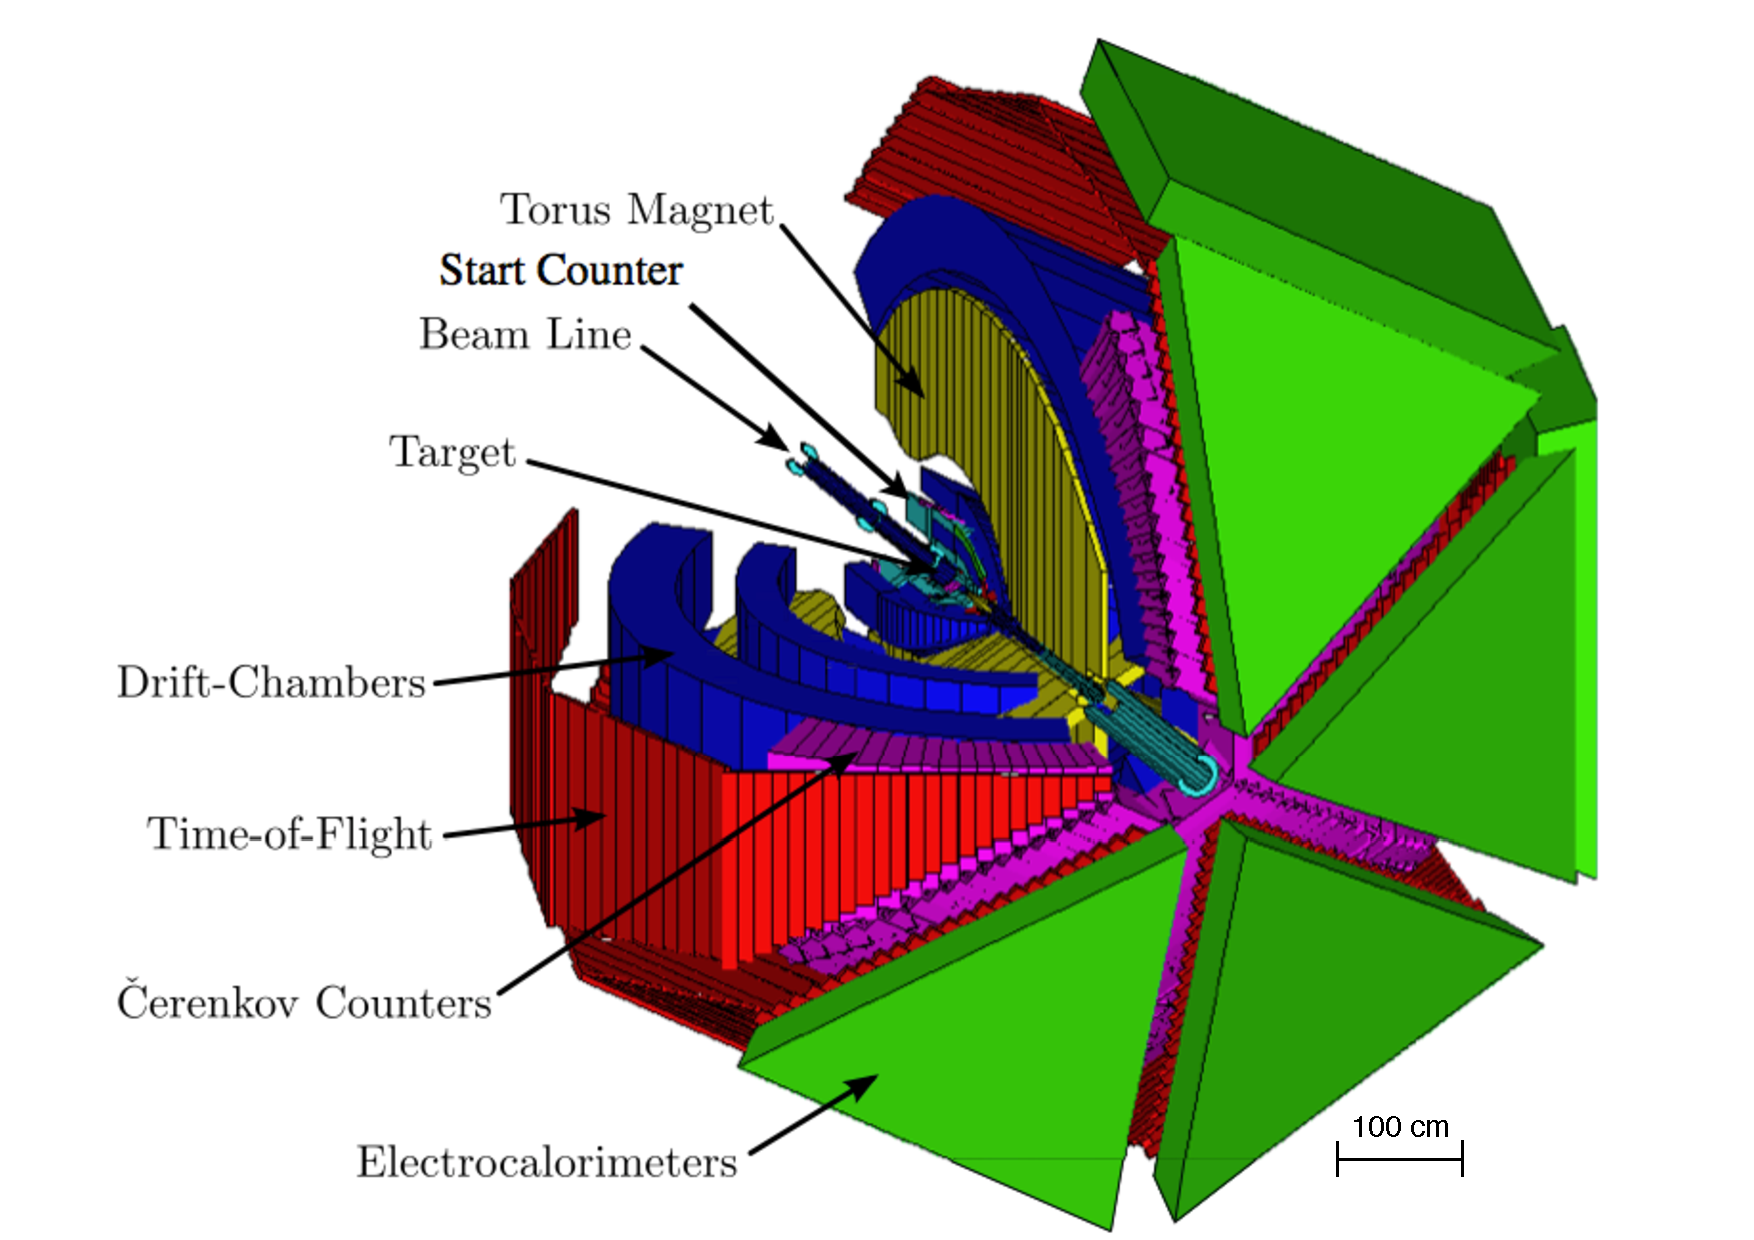
\includegraphics[width=175 pt]{figures/clas_schematicIII.pdf}}
	\caption{The CEBAF Large Acceptance Spectrometer (\textsc{\texttt{CLAS}}) }
	\label{fig:clas}
\end{figure}
\section{The g12 Experiment}
The \g12 experiment is a photoproduction experiment, it ran during March - June 2008 with a total of 44 days of good beam time. It collected over 128~TB of raw data that consisted of $26\cdot 10^9$ events, with an integrated luminosity of 68~pb$^{-1}$. The photon beam was produced by impinging a $5.715$~GeV electron beam, at 65nA, on a Au radiator of $10^{-4}$ radiation length. Photons in the energy range from 20\% to 95\% of the electron beam
energy were tagged, resulting in a photon beam energy range of 1.1-5.5~GeV. This photon beam was then collimated before being introduced onto a $\ell H_2$ target 40~cm in length along the z-direction and 2~cm radius. The placement of the target was 90~cm upstream from \abbr{CLAS} center (toward Au radiator), this increased the acceptance of particles in the forward direction. During the runtime of \g12, the Cherenkov detectors were filled with perfluorobutane ($\mathrm{C_4F_{10}}$) allowing for electron/positron detection. The experiment had a dedicated trigger, amongst 9 other triggers, that consisted of \abbr{CC} and \abbr{EC} coincidence hits for the entire beam energy range. With proper cuts on the \abbr{CC} and \abbr{EC} a $\pi/e$ rejection of $10^6$ for $e^{\pm}$ pairs was established.
\subsection{Particle Selection}
Particle selection consisted of all beam photons that were within 1.002~ns timing coincidence of the event, 1 proton and 2 oppositely charged tracks that were not the proton. This selection is appropriate for identifying the $\pi^0 \to e^+e^-\gamma$ decay because the mass of the $\pi^0$ is less than that of $\pi^{\pm}$, meaning $\pi^0$ cannot decay into $\pi^{+}\pi^{-}$.
\subsection{Kinematic Cuts}
First it should be noted that for the /g12 experiment, there was a two-prong trigger for events in which the photon beam energy was greater then 3.6~GeV, while for the entire data taking process there was a ``lepton'' trigger configuration. Therefore to measure the differential cross-section at photon beam energies less than 3.6~GeV this ``lepton'' trigger information was employed. 
Once particle section was achieved, it was necessary to reduce the background of the exclusive $\gamma p \to p \pi^{+}\pi^{-}$ reaction. For events of photon beam energy less than 3.6~GeV, a \abbr{CC} and \abbr{EC} ``hit'' must have been recorded for each charge track that was not the proton. For all events 3 kinematic fits were performed, a 1-C ( $\gamma p \to p e^{+}e^{-}(\gamma)$) to identify the missing photon in the reaction, a 4-C ($\gamma p \to p \pi^{+}\pi^{-}$) as a discriminator and a 2-C ($\gamma p \to p \pi^0 \to pe^{+}e^{-}(\gamma)$) to identify the reaction. After the kinematic fit, a 1\% confidence level cut was placed on the 1-C fit. The missing energy of the $\gamma p \to p e^{+}e^{-}$ spectrum versus the missing mass of $\gamma p \to p X$ was analyzed and shown that a 75~MeV cut on the missing energy was suitable to suppress the $\gamma p \to p \pi^{+}\pi^{-}$ reaction, see figure~\ref{fig:Mxp}. After the missing energy cut, the signal to background ratio was $\sim 99.7\%$, see right figure~\ref{fig:Mxp}, the other 4-C and 2-C fits were then used with a 1\% confidence on each to suppress the background to $\sim 99.9\%$.
\begin{figure}[h!]
	\centering
	\begin{minipage}{.50\textwidth}
		\centering
		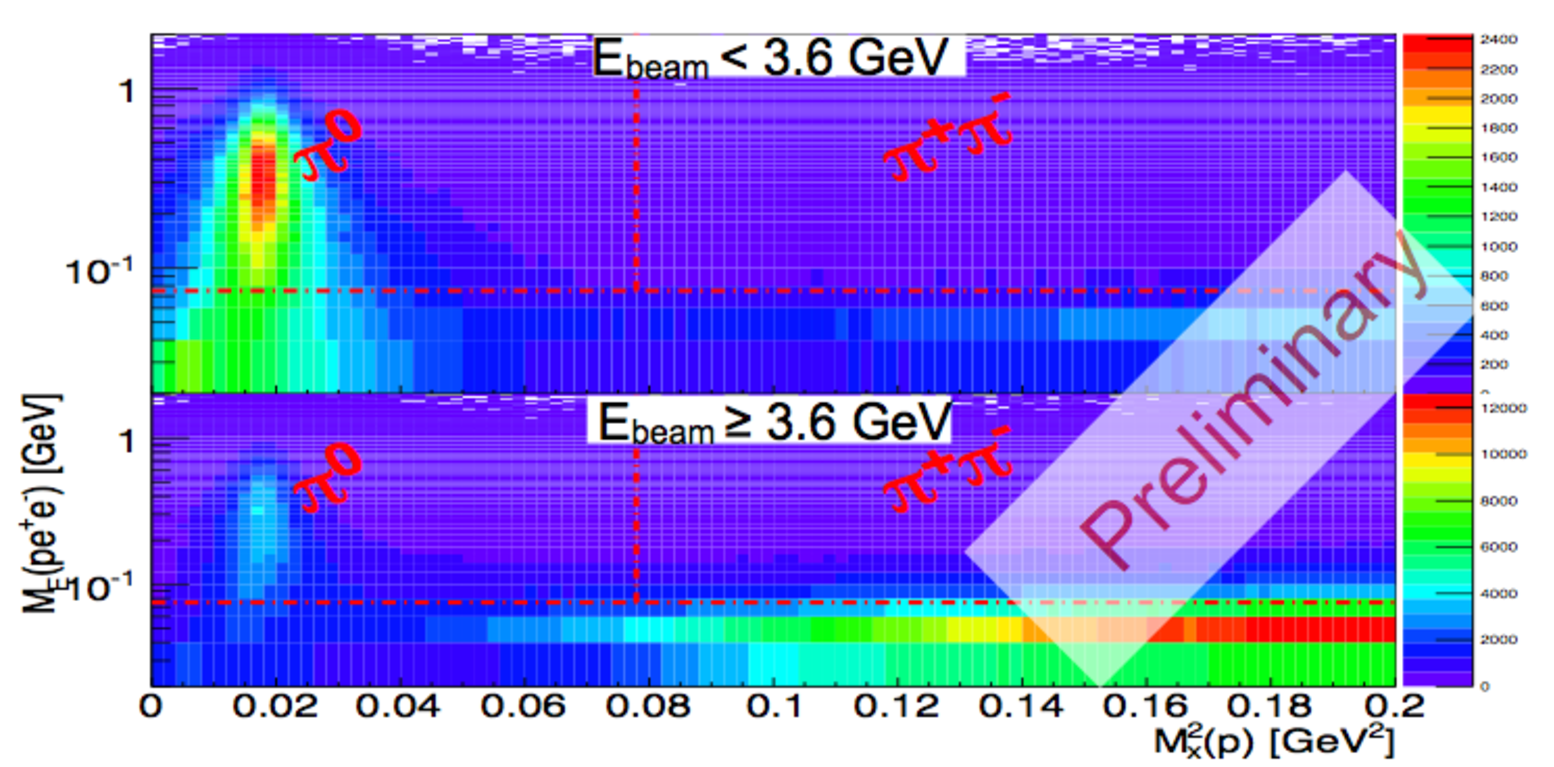
\includegraphics[width=225 pt, height = 150 pt]{figures/pi0_ME_vs_Mx.pdf}
		\caption{}{}
		\label{fig:Mx_ME}
	\end{minipage}%
	\centering
	\begin{minipage}{.50\textwidth}
		\centering
		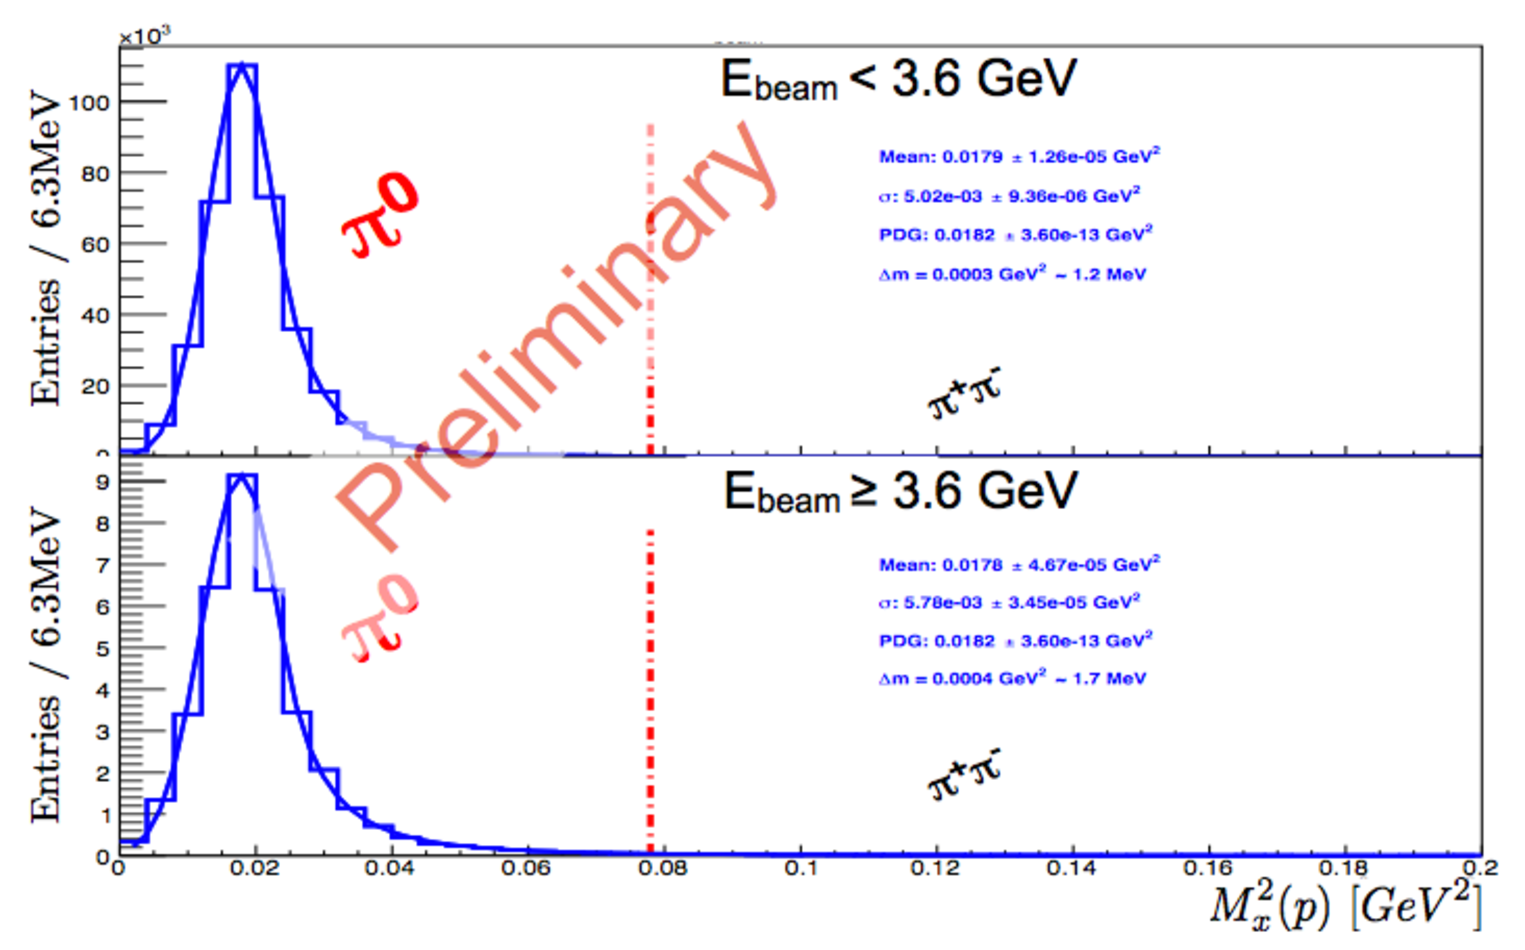
\includegraphics[width=225 pt, height = 150 pt]{figures/pi0_spectrum.pdf}
		%\caption{figure in here}{box diagram}
		\caption{Left: $M_x^2 (p)$ vs. $M_E(pe^+e^-)$. The horizontal red dashed-dotted line depicts the 75 MeV cut used in this analysis. The vertical red dashed-dotted line depicts the boundary of single $\pi^0$ to $\pi^{+}\pi^{-}$ production. Right: Final $M_x^2(p)$ data used in analysis. The horizontal red dashed-dotted line depicts the threshold of $\pi^{+}\pi^{-}$ production.}{}
		\label{fig:Mxp}
	\end{minipage}
\end{figure}
\section{Comparison to Existing Data}
There has been multiple measurements of the $\pi^0$ cross-section in single pion photoproduction that can be compared to \g12 measurements~\cite{Dugger07,ELSA05,ELSA11,Graal,LEPS,brem}, however no experiment has produced the cross-section continuously at beam energies greater than 3~GeV. Furthermore there exists solutions to partial wave analysis and databases that can predict the behavior of production of $\pi^0$ based upon previous data~\cite{BonnGat,SAID}. In figure~\ref{fig:pi0II} a comparison of the \g12 measurement is shown along with measurements from past results as well as the SAID and Bonn-Gatchina partial wave solutions. As it can be seen the \g12 data agrees well with previous measurements. This agreement gives confidence to the \g12 measurements at not previously measured beam energies. 
\begin{figure}[h!]
	\centering
	\begin{minipage}{.50\textwidth}
		\centering
		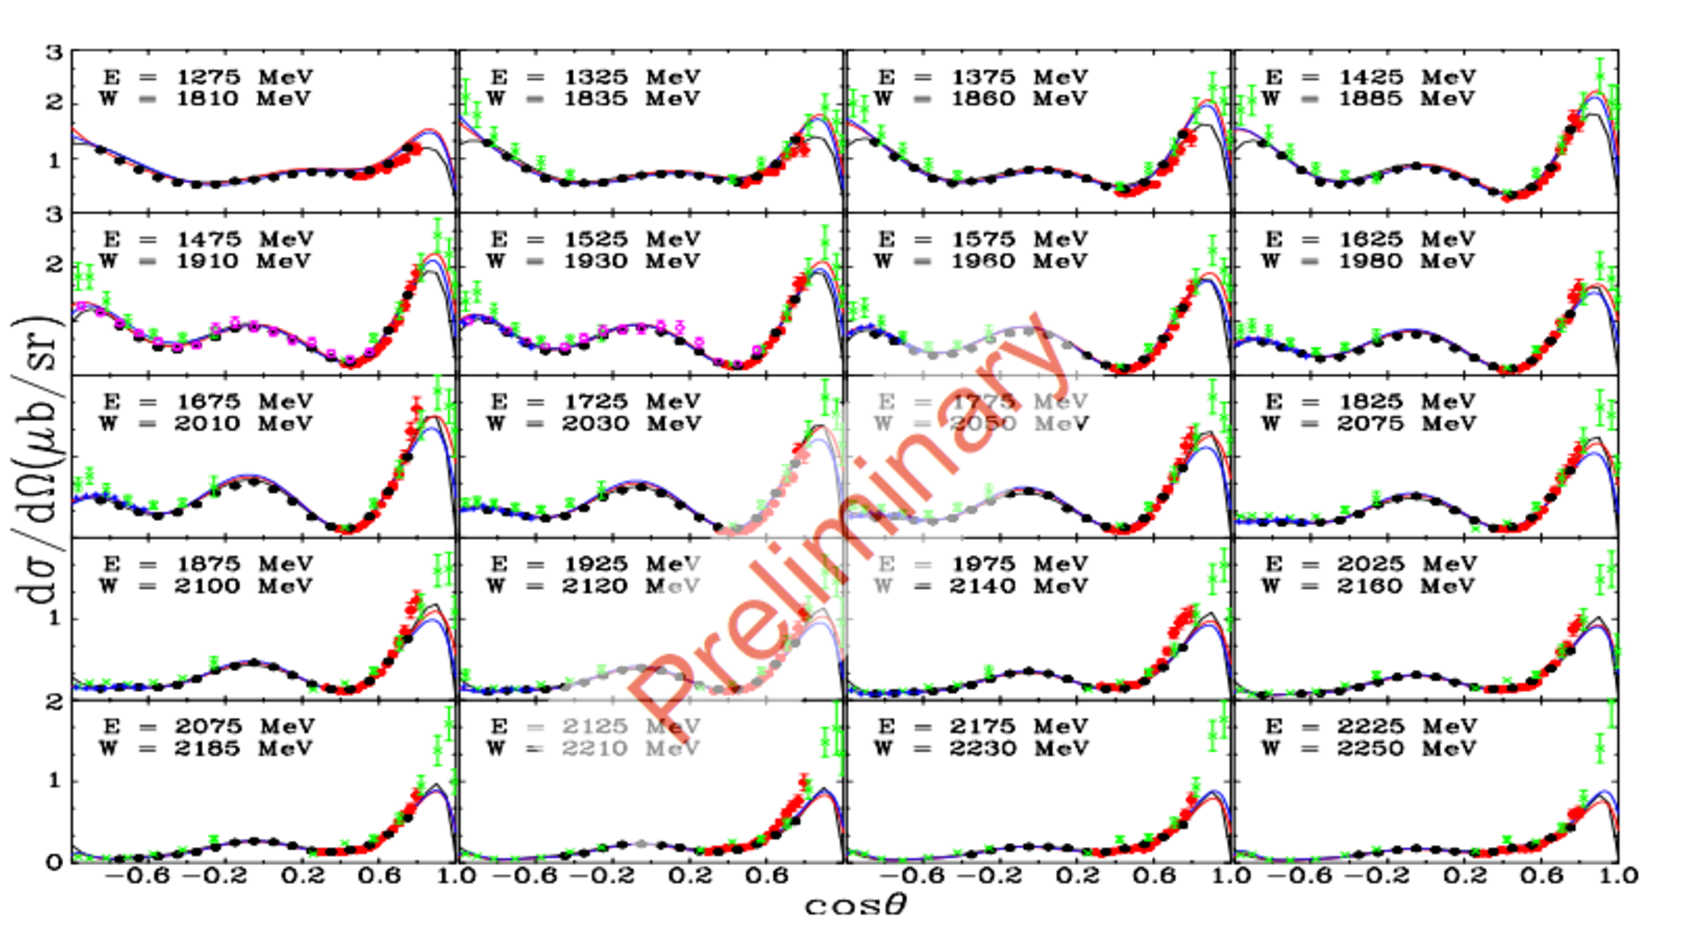
\includegraphics[width=225 pt, height = 160 pt]{figures/pi0_xsectionI.pdf}
		\caption{}{}
		\label{fig:pi0I}
	\end{minipage}%
	\centering
	\begin{minipage}{.50\textwidth}
		\centering
		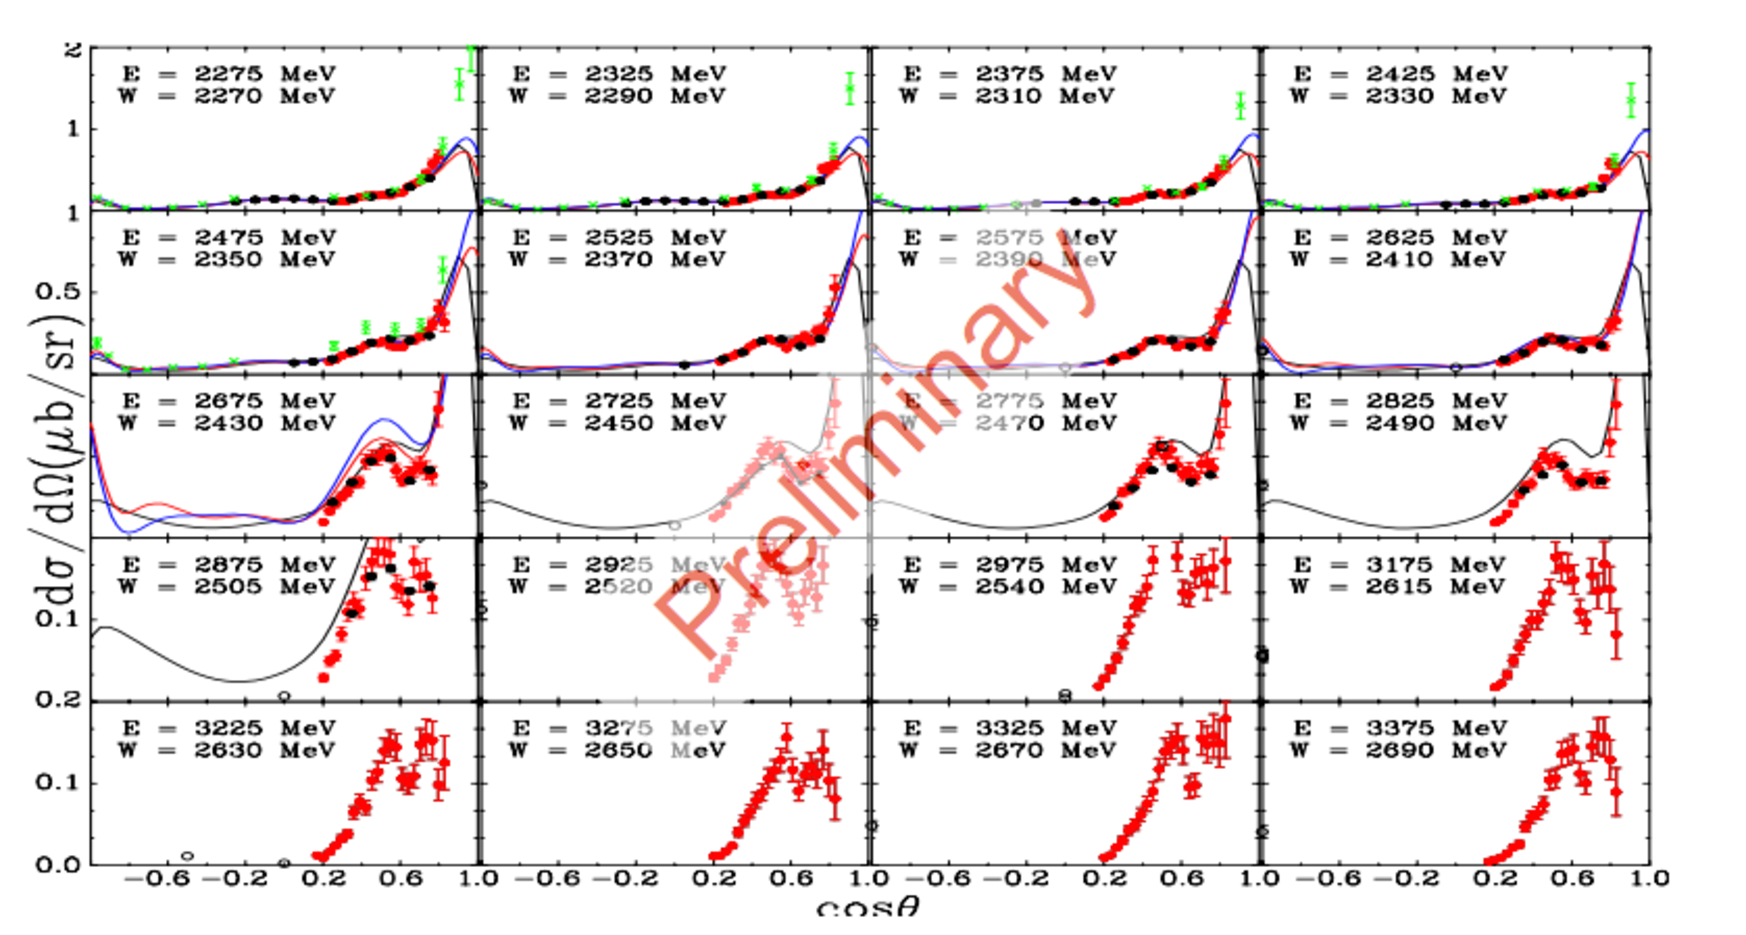
\includegraphics[width=225 pt, height = 160 pt]{figures/pi0_xsectionII.pdf}
		%\caption{figure in here}{box diagram}
		\caption{(Color online)The $\pi^0$ proton photoproduction cross section, $(d\sigma/d\Omega)$, at $E_{\gamma}$ = 1.275 -- 2.225~GeV(right):$E_{\gamma}$ = 2.275 -- 3.375~GeV(left) versus $\cos\theta$ where $\theta$ is the pion center-of-mass production angle. Photon energy is indicated by $E$, while the center-of-mass total energy is indicated by $W$. Red solid (blue solid) lines show the SAID KU14 (DU13~\protect\cite{Dugger13}) calculations. Black solid lines give the BG2011-02 BnGa~\protect\cite{BonnGat}) predictions. Experimental data are from the current measurement (red filled circles), CLAS~\protect\cite{Dugger07} (black filled circles), GRAAL~\protect\cite{Graal} (magenta open circles), LEPS~\protect\cite{LEPS} (blue plus), CB-ELSA~\protect\cite{ELSA05}~\cite{ELSA11} (green crosses). Plotted uncertainties are statistical. The plotted points from previously published experimental data are those data points within $\pm$3~MeV of the photon energy indicated on each panel.}{}
		\label{fig:pi0II}
	\end{minipage}
\end{figure}
\subsection{Comparison to Theory}
There are several models that attempt to describe  $\pi^0$ photoproduction in the low beam energy resonance region, while in the high beam energy regime there exists limited amount of theory. Described below are two theories. 
\subsubsection{HandBag Model}
The production of the \piz meson in photon-proton reactions, for incoming photon beam energies greater than 2.8~GeV, can considered to be a hard exclusive reaction. One approach to study the \piz photoproduction, is use the handbag model. In the handbag approach, the reaction is factorized into two parts. The first part is when one quark from the incoming and one from the outgoing nucleon participate in the hard sub-process. This hard sub-process is achieved when the incident photon excites a quark, since quarks are bound quantum particles, the excited quark produces a jet of quarks that form the meson and then de-excites back into the nucleon. This is calculable using pQCD. The second part ,the soft part, consists of all the other quarks that are spectators and can be described in terms of GPDs~\cite{key1, key2,Rad1996, Diehl}. The handbag mechanism is applicable when the Mandelstam variables, $s$, $t$, $u$, are large as compared to a hadronic scale of order 1 GeV . In Ref.~\cite{Huang2000} a model, derived from the handbag approach, has been applied to predict angular dependence of scaled photoproduction cross section of \piz and is illustrated in Fig.~\ref{fig:pi0_handbag}. The handbag model calculations by Kroll \textit{et al.}~\cite{Huang2000} does not agree with the measurement obtained by \g12.
\begin{figure}[h]
	\centerline{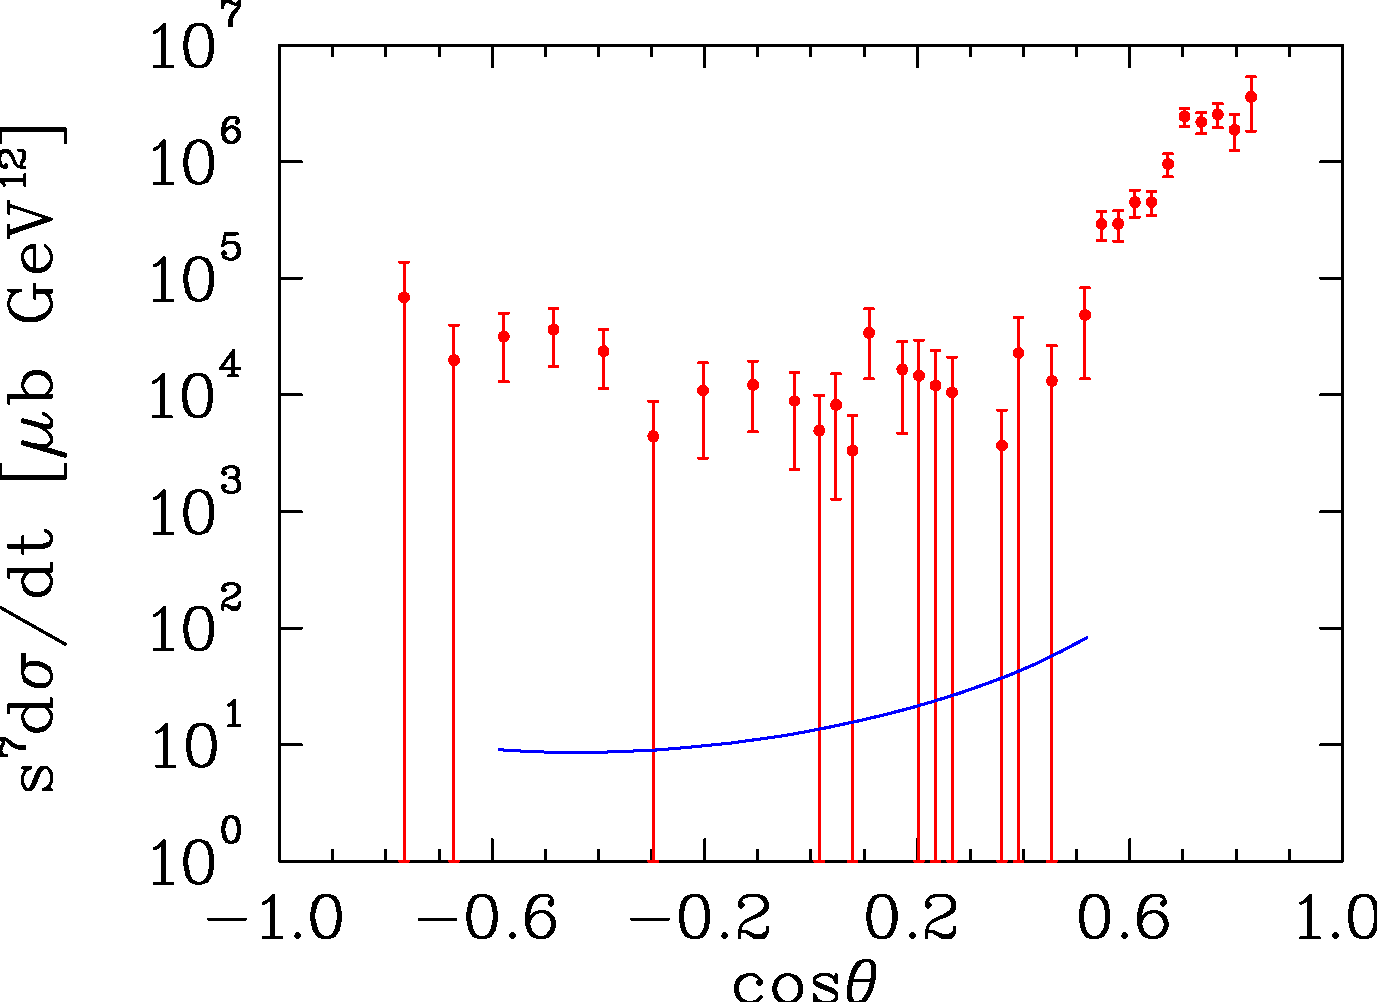
\includegraphics[width=200 pt]{figures/kroll-eps-converted-to.pdf}}
	\caption{Comparison of the $\pi^0$ differential cross section  photoproduction data to \abbr{GDP} handbag model. Experimental data at $s$ = 11.08~GeV$^2$ are from the current (red filled circles). The theoretical prediction at $s$ = 10~GeV$^2$ by Kroll \textit{et al.}~\protect\cite{Huang2000} is given by blue solid line.}
	\label{fig:pi0_handbag}
\end{figure}
\subsubsection{Regge Theory}
Another approach to describe the production of the \piz meson in photoproduction is to use Regge theory. According to Regge theory the reaction amplitudes can be described by Regge poles in which the dominant Regge poles originate from t-channel exchange. This model has been developed over the years and is greatly described in~\cite{JPAC}. Using this model along with the \g12 measurements, seen in figure~\ref{fig:pi0_regge}, it is shown that this theory provides a good description of the data obtained by \g12 and a previous measurement~\cite{brem}.
\begin{figure}[h]
	\centerline{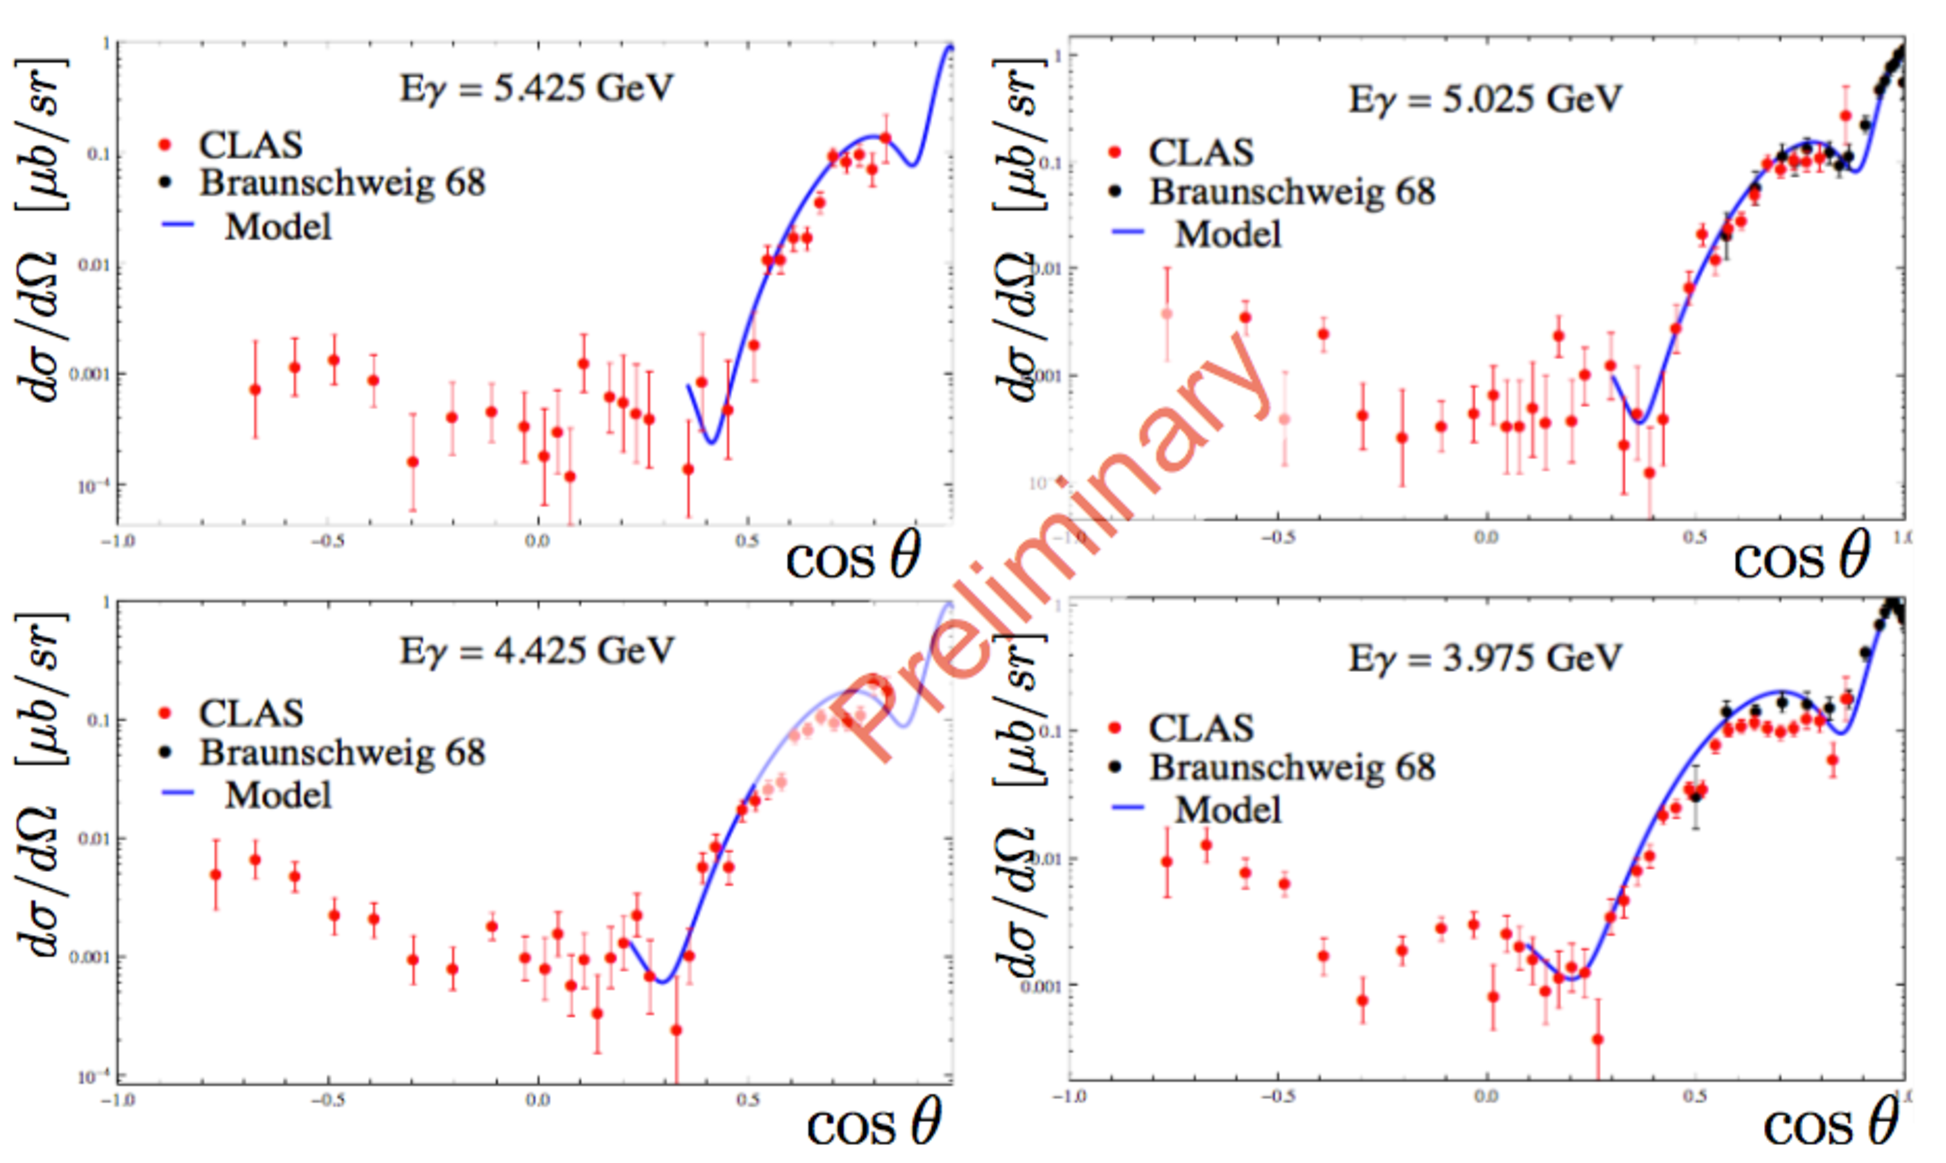
\includegraphics[width=275 pt, height = 160 pt]{figures/pi0_regge.pdf}}
	\caption{Comparison with Regge model. Experimental data are from the current measurement (red filled circles) and previous bremsstrahlung measurements~\protect\cite{brem} (black open circles). }
	\label{fig:pi0_regge}
\end{figure}
\subsection{Constituent Counting Rule}
The constituent counting rule (CCR) predicts the energy dependence of the differential cross-section at fixed center-of-mass angles for an exclusive two-body reactions. It validity is at high beam energies and large momentum transfer and the framework is similar to that of the handbag approach, in which the theory relies on the factorization of the exclusive process into a hard scattering amplitude and a soft quark amplitude inside the hadron. The prediction of CCR is:
\begin{equation}
\frac{d\sigma}{dt} \sim s^{2-n}f(\theta_{c.m.}) \label{CCR}
\end{equation}
where $s$ and $t$ are the Mandelstam variables, $n$ is the total number of interacting elementary fields in the initial and final state of the reaction and $f(\theta_{c.m.})$ depends on the dynamics of the process. Many exclusive measurements in $pp$ and  $\bar{p}p$ elastic scattering~\cite{scalingexp5, scalingexp7}, meson-baryon $M p$ reactions~\cite{scalingexp7}, and photoproduction $\gamma N$~\cite{scalingexp2, scalingexp3, scalingexp4, scalingexp6, scalingexp8, scalingexp9, scalingexp10, scalingexp11} agree well with this rule. For \piz photoproduction reactions CCR predicts that the differential cross-section $\frac{d\sigma}{dt}$ should scale as $s^{-7}$, where -7 was calculated from 4 elementary fields in the initial state, 1 for the photon, 3 for the number of quarks in a proton, and 5 elementary fields in the final state, 3 quarks from the proton and  2 quarks from the \piz, 2-9 =-7. A comparison of this previous data along with the \g12 measurements can be seen in figure~\ref{fig:pi0_scaling}, at high energies and large angles the results are consistent with the $s^{−7}$ scaling expected from the quark counting rule. 
\begin{figure}[h]
	\centerline{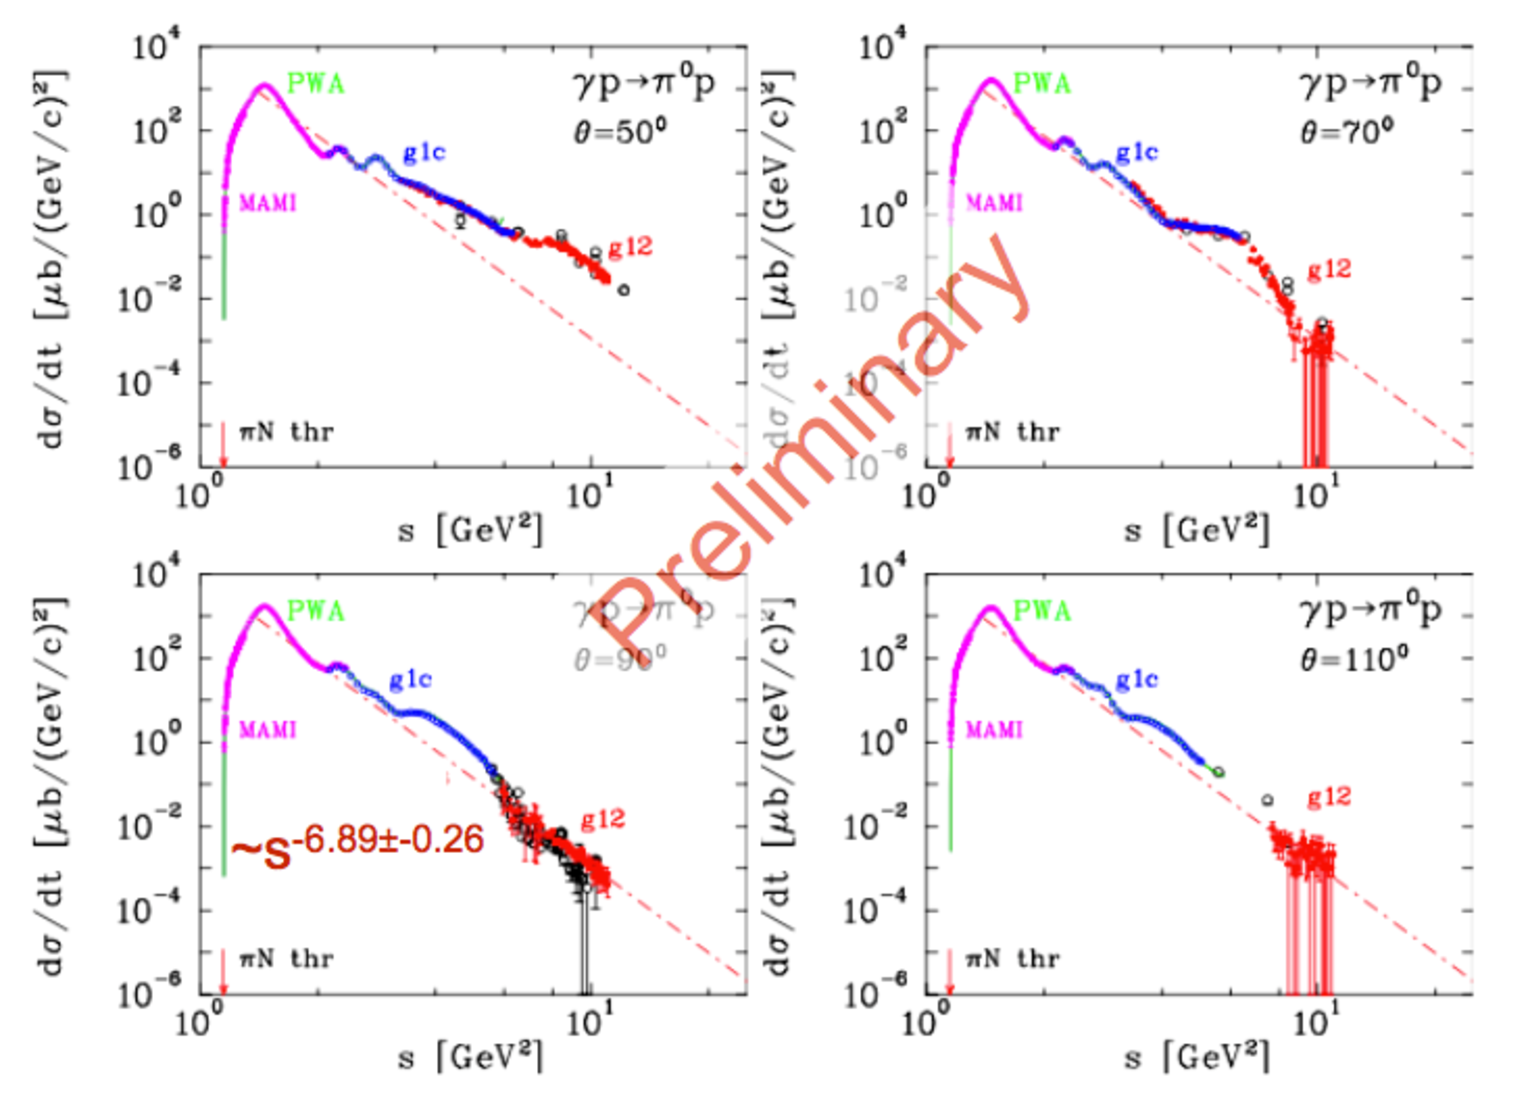
\includegraphics[width=250 pt]{figures/pi0_scaling.pdf}}
	\caption{The differential cross section for the $\gamma p \to p \pi^0$ reaction at $\theta_{c.m.}$ = $50^{\circ}$, $70^{\circ}$, $90^{\circ}$, $110^{\circ}$, as a function of s (center of mass energy squared). Experimental data are from the current measurement (red filled circles), CLAS~\protect\cite{Dugger07,Dugger13} (blue circles), MAMI~\protect\cite{beck} (magenta circles), old measurements~\protect\cite{Joos} (black open circle plus). The dash dotted line is a result of the fit performed at $\theta$ = $90^{\circ}$ with power function $\sim s^{−n}$ leading to n = $6.89 \pm 0.26$.}
	\label{fig:pi0_scaling}
\end{figure}
\subsection{HALL C at Jlab12 Outlook}
The newly upgraded Hall C at Jefferson Lab will perform an experiment to measure \piz photoproduction cross-section on a $\ell H_2$ target. The experiment will be set up to measure \piz from $70^{\circ}<\theta_{c.m.}<110^{\circ}$ in the photon beam energy range of 6--10~GeV. The recoiled protons will be detected in the High-Momentum Spectrometer (HMS) while the photons from \piz decay will be detected by the Neutral Particle Spectrometer(NPS) as seen in figure~\ref{fig:hallc12}.
\begin{figure}[h]
	\centerline{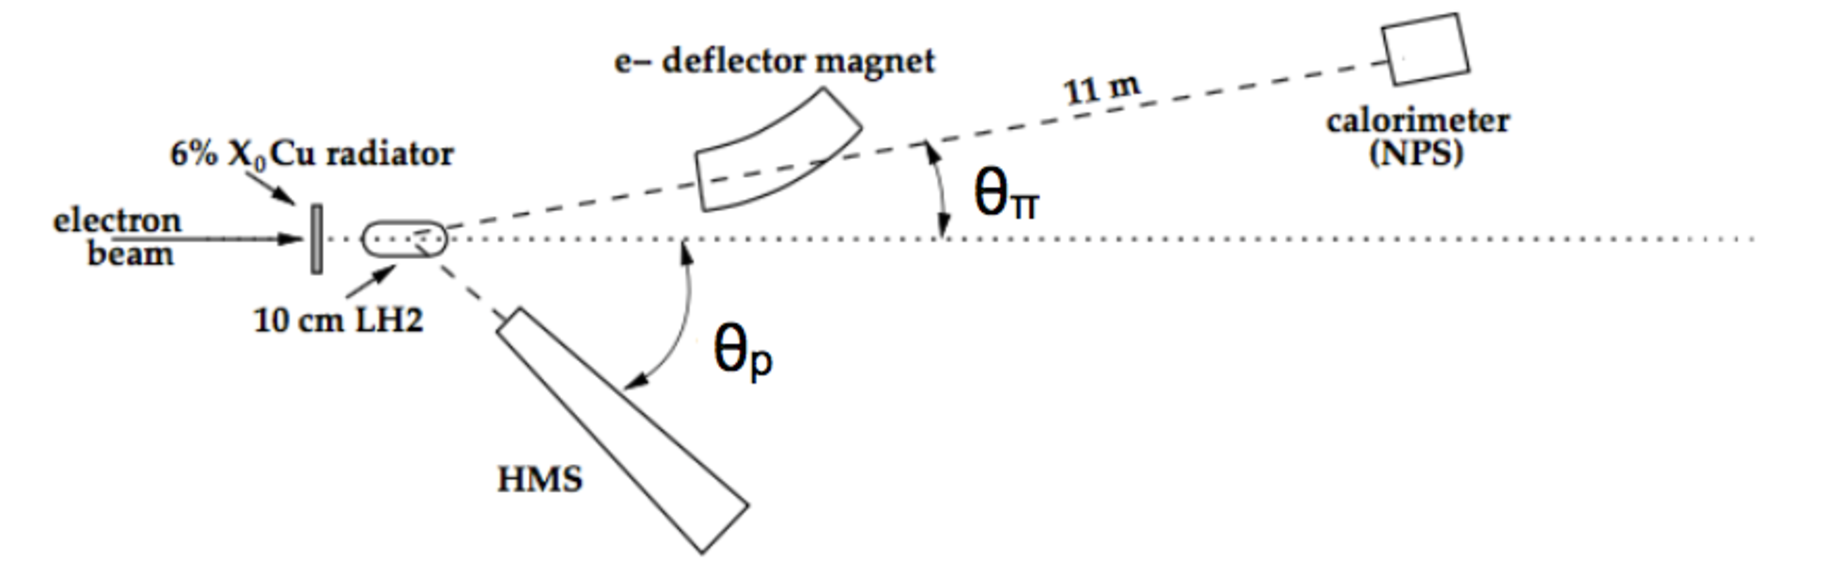
\includegraphics[width=250 pt, height = 100 pt]{figures/HALLC12.pdf}}
	\caption{Hall C setup at 10~GeV with the HMS detecting the recoil protons and the phtoon calorimeter detecting the scattered photons from the \piz decay. }
	\label{fig:hallc12}
\end{figure}
The projected measurements to be taken at Hall C as well as previous measurements can be seen in figure~\ref{fig:pi0_projected}.
\begin{figure}[h]
	\centerline{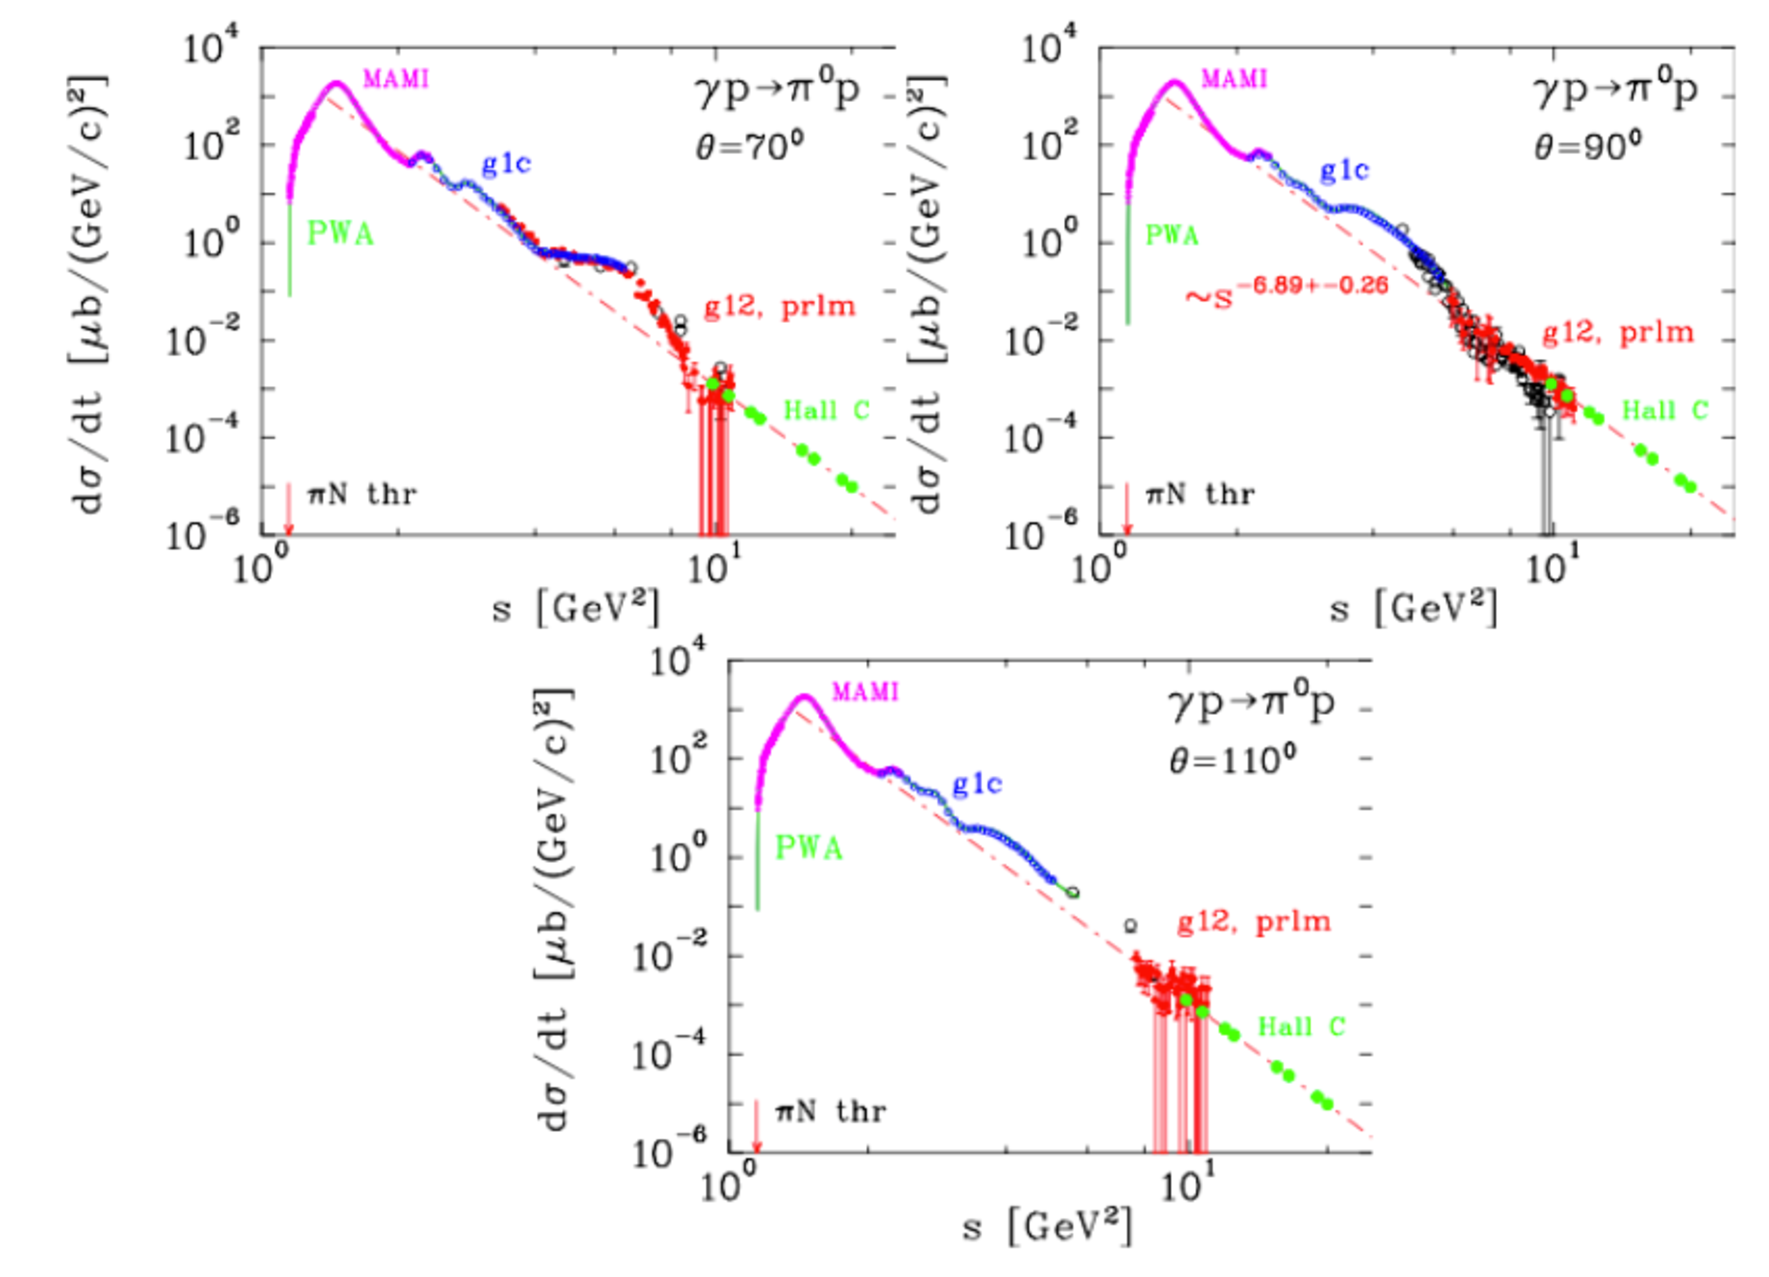
\includegraphics[width=300 pt, height = 160 pt]{figures/HallC_projected.pdf}}
	\caption{The differential cross section for the $\gamma p \to p \pi^0$ reaction at $\theta_{c.m.}$ = $50^{\circ}$, $70^{\circ}$, $90^{\circ}$, $110^{\circ}$, as a function of s (center of mass energy squared). Experimental data are from the current measurement (red filled circles), CLAS~\protect\cite{Dugger07,Dugger13} (blue circles), MAMI~\protect\cite{beck} (magenta circles), old measurements~\protect\cite{Joos,Fuchs} (black open circle plus), projected Hall C results(green circles). }
	\label{fig:pi0_projected}
\end{figure}
\newpage
% Acknowledgement
% References

\nocite{*}
\bibliographystyle{aipnum-cp}%
\bibliography{PI0}%


\end{document}
